\chapter{Digital sampling}
We studied how to reconstruct a signal starting from its sampling. We tried different sampling frequencies and two different waves then using the Whittaker–Shannon formula we have reconstructed the orginal signal. 

\section{Materials}
\begin{itemize}
\item Waveform generator RIGOL DG1032
\item National Instruments myDAQ
\end{itemize}
\section{Experimental setup}
The waveform generator and the NI myDAQ were connected togheter so that we could use the LabView software for aquiring the data. The sampling frequency and the number of samples were set with the software. As source signal we used a sine wave with $10$ Hz frequency and a pk-pk amplitude of $5$ V. We sampled this wave with a frequency of 5, 10 and 25 Hz. We then changed the wave with a triangular one of 100 Hz and 4 V pk-pk amplitude: this last signal was sampled with a 500 Hz frequency only.
\section{Data analysis}
The Whittaker–Shannon formula states that:
\[x(t) = \sum_n x_n\cdot\text{sinc}\left(\frac{t-t_n}{T}\right)\]
where $x_n$ are the data corresponding to the time $t_n$ and $T$ is the sampling period.
There is however a limit to its application: the results from this formula are significant only if the sampling frequency is higher than two times the highest one present in the signal. In the following plots in fact can be easily verified this principle: the original signal is well reconstructed only when we had a sampling frequency higher than 2 times the signal one. 
\begin{figure}[H]
\centering
\begin{minipage}{.5\textwidth}
  \centering
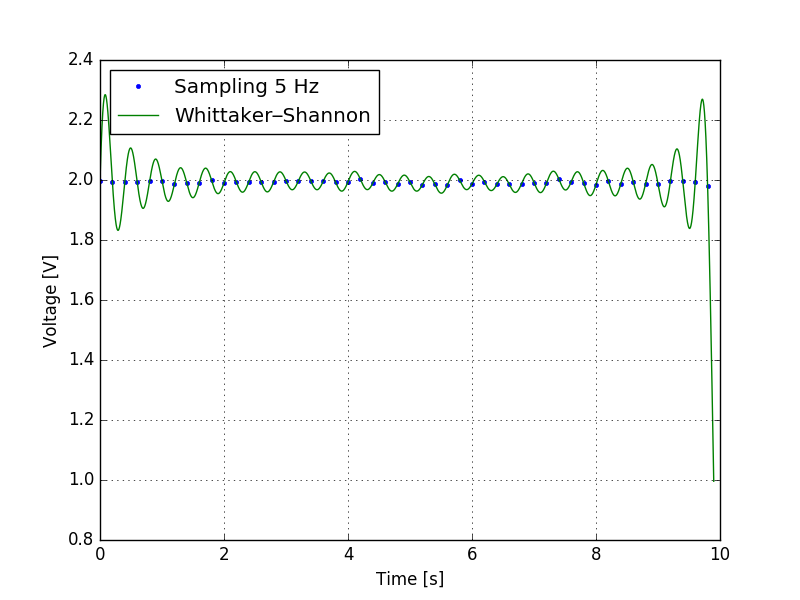
\includegraphics[width=\textwidth]{13/5Hz.png}
\caption{Sine input, sampling frequency: 5 Hz}
\end{minipage}\hfill
\begin{minipage}{.5\textwidth}
  \centering
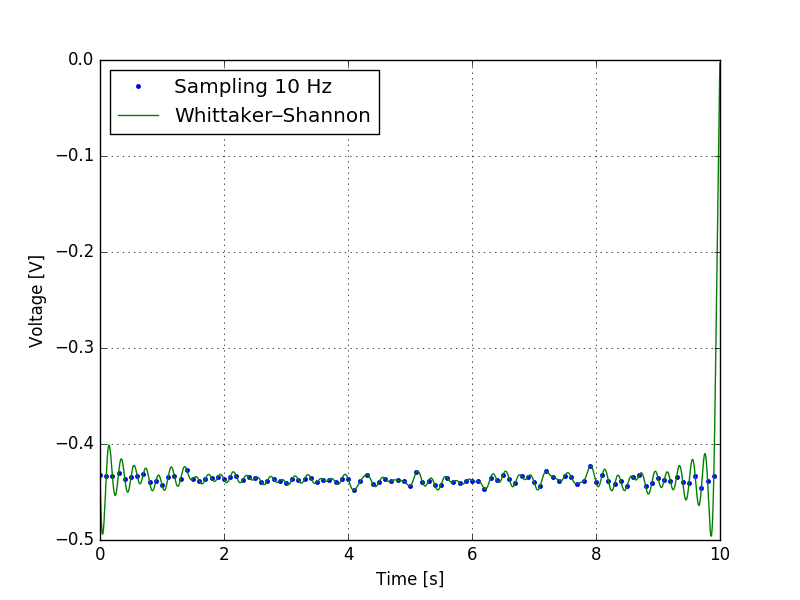
\includegraphics[width=\textwidth]{13/10Hz.png}
\caption{Sine input, sampling frequency: 10 Hz}
\end{minipage}
\end{figure}
\begin{figure}[H]
\centering
\begin{minipage}{.5\textwidth}
  \centering
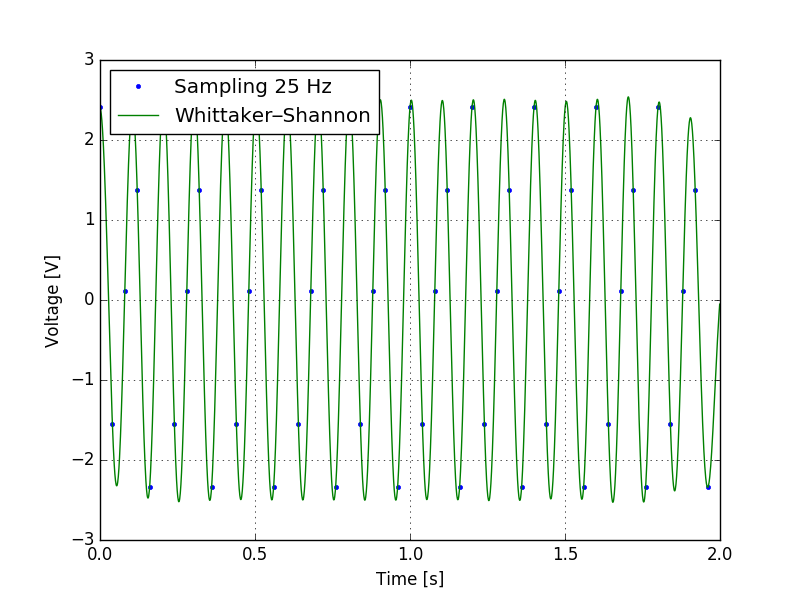
\includegraphics[width=\textwidth]{13/25Hz.png}
\caption{Sine input, sampling frequency: 25 Hz}
\end{minipage}%
\begin{minipage}{.5\textwidth}
  \centering
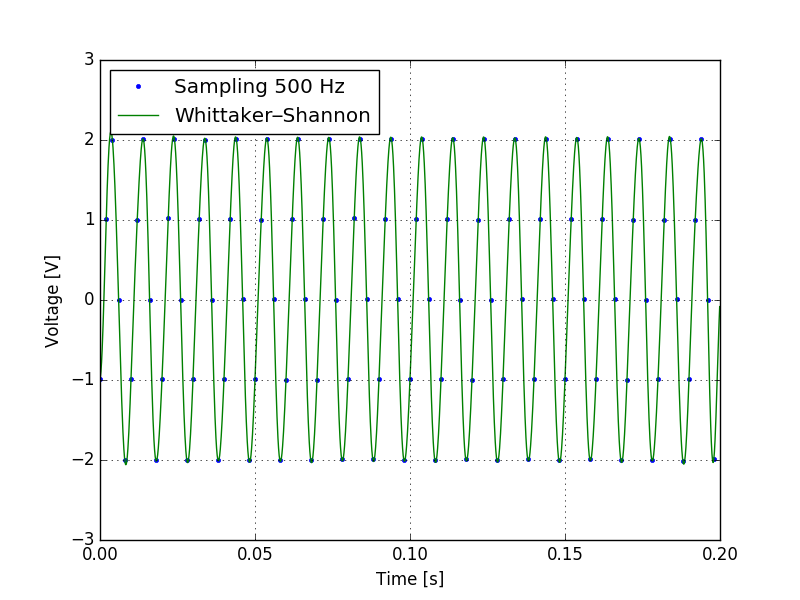
\includegraphics[width=\textwidth]{13/500Hz.png}
\caption{Triangular input, sampling frequency: 500 Hz}
\end{minipage}
\end{figure}
